\documentclass{article}
\usepackage[a4paper,margin=1in]{geometry}
\usepackage{amsmath, amsfonts, amssymb, amstext, mathtools, stmaryrd, textcomp, xcolor, graphicx, tikz}
\usepackage[hidelinks]{hyperref}
\usetikzlibrary{automata, positioning, arrows, trees}
\tikzset{->,>=stealth,
every state/.style={thick, fill=gray!10}, 
initial text=$ $,
}
\newcommand{\answer}{\textcolor{red}}
\newcommand{\e}{\varepsilon}
\newcommand{\s}{\Sigma}
\newcommand{\g}{\Gamma}
\newcommand{\so}{\rightarrow}
\newcommand{\str}{\texttt}
\newcommand{\newp}{\\[2mm]}
\newcommand{\defeq}{\coloneqq}
\newcommand{\spc}{\textvisiblespace}

\title{Homework 06}
\author{Aaron Wang}
\date{March 28 2025}

\begin{document}
\maketitle
\begin{enumerate}
    \item \textbf{Doubly infinite tapes} [Problem 3.11]. A Turing machine with a doubly infinite tape is like a TM as defined in the book, but with a tape that extends infinitely in both directions (not just to the right). Initially, the head is at the first symbol of the input string, as usual, but there are infinitely many blanks to the left. Show how, given a TM with doubly infinite tape, to construct an equivalent standard TM. An \textbf{implementation description} in the style of Proof 3.13 is fine, and it’s also fine to use any results proved in the book or in class. \newp
    \answer{
    Let NEURAL$ = \{ \langle N \rangle \:|\: N$ is a \emph{neural network} and there exists inputs $x_1,...,x_l$ that make $y = 1\}$.\newp
    % To prove NEURAL is NP-complete, we must show it is both NP and NP-hard.\newp
    Let $V$ be a verifier for NEURAL.\newp
    $V =$ ``On input $\langle N, X \rangle$ where $N$ is a neural network and $X$ is the sequence of inputs $x_1,...,x_l$:
    \begin{enumerate}
        \item [1.] $\forall j$ solve $h_j$.
        \item [2.] Solve $y$.
        \item [3.] If $y = 1$, \emph{accept}; otherwise, \emph{reject}.
    \end{enumerate}
    Step 1 is $\mathcal{O}(l*m)$ and step 2 is $\mathcal{O}(m)$. Consequently, $V$ is definitely $\mathcal{O}(n^2)$. Since we have a deterministic polynomial time verifier, we know NEURAL is NP.\newp
    Here are the details of a reduction from 3SAT to NEURAL that operates in polynomial time.
    \begin{enumerate}
        \item [1.] Initialize nodes for $x_i$ and $\overline{x_i}$ s.t. they must be opposites. For each variable $x_i$:
        \begin{itemize}
            \item Create nodes $x_i$ and $x_{-i}$
            \item Create node $h_{x_i} = H(x_i+x_{-i})$
            \item Create node $h_{x_{-i}} = H(-x_i-x_{-i}+2)$
        \end{itemize}
        \item [2.] Translate all the clauses into the neural network. For each clause $j$: create $h_j$ s.t. 
        \begin{itemize}
            \item if $x_i$ is in the clause, $u_{i,j} = 1$
            \item if $\overline{x_i}$ is in the clause, $u_{-i,j} = 1$
            \item otherwise $u_{i,j} = 0$
        \end{itemize}
        \item [3.] And every clause (step 2) and restriction (step 1) together. $\displaystyle y = H(\sum_{j=1}^mh_j - m + 1)$
    \end{enumerate}
    Following this reduction, we have mapped each boolean expression to a neural network that is satisfiable iff the boolean expression is. Every $N$ that is made from this reduction will only be satisfiable, if there is a series of inputs that make every $h = 1$ or all clauses and restrictions are satisfied 
    Step 1 is $\mathcal{O}(n)$, 2 is $\mathcal{O}(n^2)$, and 3 is $\mathcal{O}(n)$. This is clearly a $\mathcal{O}(n^2)$ reduction so NEURAL is NP-Hard.\newp
    Since NEURAL is NP and NP-Hard, it is NP-complete.
}
%
    \item \textbf{Two-stack PDAs}. A \emph{two-stack pushdown automaton} (2PDA) is a pushdown automaton with two stacks. Show that any Turing machine M can be converted into an equivalent 2PDA $P$.\newp
    \textcolor{red}{
    The intuition for the following CFG is this. We need to design a CFG that accepts only balanced strings and every balanced string. This CFG clearly only accepts balanced strings as it only adds \str{0} and \str{1} simultaneously. 
    Now for the other half, a balanced string must fall into at least one of two categories. 
    The first is that $w=\str{0}x\str{1}$ or $w=\str{1}x\str{0}$ s.t. $x$ is a balanced string (it is composed of a balanced substring wrapped by \str{0} and \str{1}). 
    The other is $w=xy$ s.t. $x$, $y$ are balanced strings (It is a concatenation of two balanced substrings).
    Both of these cases are covered by the following CFG.\newp
    CFG for C with starting state $S$.
    \begin{align*}
    S &\rightarrow \str{0}S\str{1} \:|\: \str{1}S\str{0} \:|\: SS \:|\: \e
    \end{align*}
    The intuition for the following PDA is this. At each occurence of a character, we either pop the opposing character off the stack (if possible) or we add the current character onto the stack. This way, the stack will always be empty\footnote{airquotes because it will contain the \$ which signifies empty stack.} if and only if an equal amount of occurences of each character exist.\newp
    \begin{figure}[h]
    \centering
    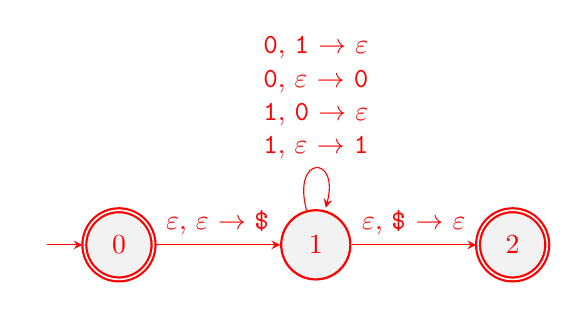
\begin{tikzpicture}
    \color{red}
        \node[state, initial, accepting] (q0) {0};
        \node[state, xshift=2.5cm] (q1) {1};
        \node[state, xshift=5cm, accepting] (q2) {2};
        \draw
        (q0) edge[] node[above]{$\e$, $\e$ $\rightarrow$ \str{\$}} (q1)
        (q1) edge[loop above] node[above, align=center]{
            \str{0}, \str{1} $\rightarrow$ $\e$\\
            \str{0}, $\e$ $\rightarrow$ \str{0}\\
            \str{1}, \str{0} $\rightarrow$ $\e$\\
            \str{1}, $\e$ $\rightarrow$ \str{1}
        } (q1)
        (q1) edge[] node[above]{$\e$, \str{\$} $\rightarrow$ $\e$} (q2)
        ;
    \end{tikzpicture}
    \end{figure}
}
    \newpage
% Use the two stacks like a tape. one stack is the front half one stack is hte back half. And you are looking at the end of the front stack. It's where "the head" of your turing machine is.
    \item Brain fun. This problem is about a programming language known as $P''$ in polite company. \newp
    Describe how to compile any $\mathcal{P}''$ program $P$ into the formal description of a Turing machine $M_P$ equivalent to $P$. The input to $M_P$ would be a string $w \in \s^*$, and it should accept iff $P$ accepts w. It should be a standard single-tape TM, but you can use S (“stay”) actions.\newp
        \answer{
    Let SAFEROOM $= \{\langle R\rangle \:|\: R$ is a room that can have a safe path$\}$\newp
    Let $V$ be a verifier for SAFEROOM.\newp
    $V =$ ``On input $\langle R, c \rangle$ where $R$ is as described above and $c$ is the certificate, a set of toggled buttons:
    \begin{enumerate}
        \item [1.] For each tile in the grid $T_{i,j}$, decide if it is closed or open
        \begin{enumerate}
            \item [i.] If $R_{i,j}$ has letter $\sigma$ and $\sigma \in c$, $T_{i,j}$ is the inverse of $R_{i,j}$'s initial state.
            \item [ii.] $T_{i,j}$ is $R_{i,j}$'s initial state otherwise.
        \end{enumerate}
        \item [2.] If the entrance tile is open, \emph{reject}
        \item [3.] Mark every tile that is  adjacent to a closed, marked tile and is also closed.
        \item [4.] Repeat step 3 until no new tiles are marked.
        \item [5.] If the exit tile is marked, \emph{accept}; otherwise \emph{reject}.
    \end{enumerate}
    This essentially figures out of each tile is open or closed based on the initial state and whether it has been toggled. It then runs a bfs and accepts if there is a path. $V$ is polynomial time bounded by the size of the rectangle. Since we have a deterministic polynomial time verifier, we know SAFEROOM is NP.\newp
    Here are the details of a reduction from 3SAT to SAFEROOM that operates in polynomial time. We will map from a boolean expression to $\langle R \rangle$ an instance of SAFEROOM .
    \begin{enumerate}
        \item [1.] Let $R$ be a room that is 3 rows by $2m+1$ columns where $m =$ the number of clauses.
        \item [2.] Set the start tile to $T_{1,1}$ where we are using a 1-based indexing.
        \item [3.] For every tile in an odd column, set the initial state to closed and do not attach a letter to it.
        \item [4.] For every clause $c_j$ that looks like $a \lor b \lor c$
        \begin{enumerate}
            \item $T_{1,2j}$ is open if $a$ is a negated variable; it is closed otherwise. Additionally, $T_{1,2j}$ has symbol of the variable.
            \item Same for $T_{2,2j}$ and $b$.
            \item Same for $T_{3,2j}$ and $c$.
        \end{enumerate}
        \item [5.] Set the exit tile to $T_{1,2j+1}$.
    \end{enumerate}
    Essentially, we have created a buffer between every clause in which you can choose which ``gate'' to go through next. We then transform the clauses into a wall of gates, which can all be crossed iff the corresponding clause was satisfiable. Further, for any certificate that solves the SAFEROOM instance, we can create certificate for 3-SAT by setting all the variables in that original certificate to false. Following this reduction, we have mapped an instance of 3SAT to SAFEROOM that is satisfiable iff the the original problem is.  This is clearly $\mathcal{O}(n)$ reduction where $n$ is the number of clauses. Thus SAFEROOM is NP-hard.\newp
    Since SAFEROOM is NP and NP-Hard, it is NP-complete.
}

\end{enumerate}
\end{document}